\chapter{Calibration, Verificiation and Validation of Quantum Devices}
\label{ch:QCVV}

\section{Introduction}
\label{sec:QCVVIntro}
In this chapter, I describe the calibration and testing of a completely
reconfigurable circuit in bulk optics. By altering the parameters in this single
experiment, we were able to simulate the action of any lossless linear optics
circuit on four modes. The architecture was motivated by (but not identical to)
the scheme described by Reck et al in \cite{reck94}. An application of this
circuit to quantum simulation is described in chapter~\ref{ch:Simulations}.

\begin{figure}
  \centering
  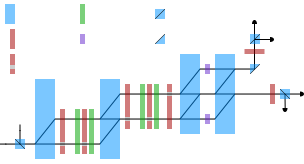
\includegraphics{figures/circuit.pdf}
  \caption[A schematic of the bulk optics circuit used for simulations.]
  {A schematic of the bulk optics circuit. Two photons are injected at
  the left of the circuit in orthogonal polarisations (\(\ket{H}\) indicates
  horizontal and \(\ket{V}\) indicates vertical), using an in-fibre polarising
  beamsplitter (PBS) to combine the two photons into a single path. The circuit
  operates in a combined path/polarisation encoding, where polarising beam
  displacers (PBD) are used to convert between the two. Operations are performed
  with fixed quarter waveplates (QWP) and polarisation flips (X), and variable
  angle half waveplates (HWP). After the operations are complete,
  polarisation-sensitive detection is performed using further PBS elements and
  single photon avalanche diodes. We label the detectors A through D.}
  \label{fig:circuit}
\end{figure}

\section{Calibration (the crapusoids are real)}
\label{sec:Calibration}
\begin{figure}
  \centering
  \begin{subfigure}{\textwidth}
    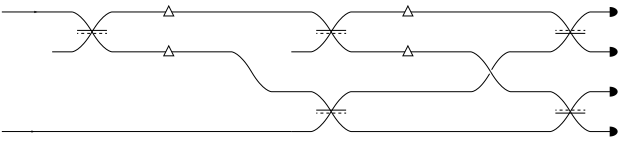
\includegraphics{figures/schematic.pdf}
    \caption{A schematic of the circuit, expanded into path}
    \label{fig:schematic}
  \end{subfigure} \\
  \vspace{1cm}
  \begin{subfigure}{0.45\textwidth}
    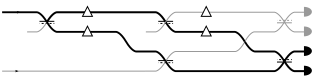
\includegraphics{figures/interferometerAB.pdf}
    \caption{A/B interferometer}
    \label{fig:ab}
  \end{subfigure}
  \hspace{0.05\textwidth}
  \begin{subfigure}{0.45\textwidth}
    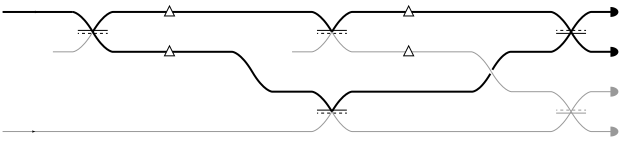
\includegraphics{figures/interferometerCD.pdf}
    \caption{C/D interferometer}
    \label{fig:cd}
  \end{subfigure}
  \caption[Illustration of nested interferometers in the bulk Reck scheme]
  {Interferometers}
  \label{fig:interferometers}
\end{figure}

\section{Benchmarking (arguably the first boson sampler)}
\label{sec:Benchmarking}

\section{Verification}
\label{sec:Verification}
Work relating to verification in quantum walks and \bosonsampling. I don't think
it's unfair to say that I had the original motivation to implement the
\(\rstar\) protocol described in \cite{aaronson13}. I did the Bayesian model
comparison between \bosonsampling and uniform distributions.
